\chapter{Geometria}

\index{geometria}

En problemes geomètrics és sovint difícil trobar una manera d'abordar
el problema de manera que la seva solució sigui senzilla d'implementar
i el nombre de casos especials sigui petit.

Per exemple, considerem un problema on se'ns donen els vèrtexs d'un
quadrilàter (un polígon amb quatre vèrtexs) i hem de calcular la seva
àrea. Una possible entrada per al problema és la següent:


\begin{center}
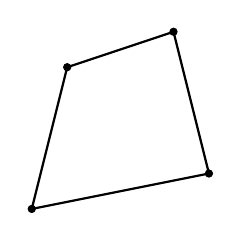
\begin{tikzpicture}[scale=0.45]

\draw[fill] (6,2) circle [radius=0.1];
\draw[fill] (5,6) circle [radius=0.1];
\draw[fill] (2,5) circle [radius=0.1];
\draw[fill] (1,1) circle [radius=0.1];
\draw[thick] (6,2) -- (5,6) -- (2,5) -- (1,1) -- (6,2);
\end{tikzpicture}
\end{center}
Una manera d'abordar el problema és dividir el quadrilàter en dos
triangles mitjançant una línia recta entre dos vèrtexs oposats:
\begin{center}
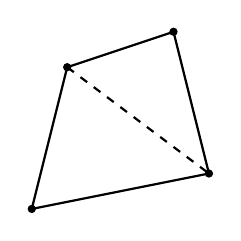
\begin{tikzpicture}[scale=0.45]

\draw[fill] (6,2) circle [radius=0.1];
\draw[fill] (5,6) circle [radius=0.1];
\draw[fill] (2,5) circle [radius=0.1];
\draw[fill] (1,1) circle [radius=0.1];

\draw[thick] (6,2) -- (5,6) -- (2,5) -- (1,1) -- (6,2);
\draw[dashed,thick] (2,5) -- (6,2);
\end{tikzpicture}
\end{center}
Després d'això, n'hi ha prou amb sumar les àrees dels
triangles. L'àrea d'un triangle es pot calcular, per exemple,
utilitzant \key{la fórmula d'Heron},
\[ \sqrt{s (s-a) (s-b) (s-c)},\]
on $a$, $b$ i $c$ són les longituds dels costats del triangle i
$s=(a+b+c)/2$. \index{Fórmula d'Heron}

Aquesta és una possible manera de resoldre el problema, però hi ha una
trampa: com dividir el quadrilàter en triangles? Resulta que de
vegades no podem escollir només dos vèrtexs contraris arbitraris. Per
exemple, en la situació següent, la línia de divisió és \emph{fora}
del quadrilàter:
\begin{center}
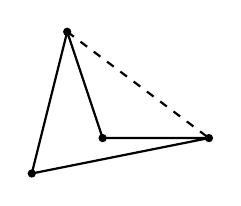
\begin{tikzpicture}[scale=0.45]

\draw[fill] (6,2) circle [radius=0.1];
\draw[fill] (3,2) circle [radius=0.1];
\draw[fill] (2,5) circle [radius=0.1];
\draw[fill] (1,1) circle [radius=0.1];
\draw[thick] (6,2) -- (3,2) -- (2,5) -- (1,1) -- (6,2);

\draw[dashed,thick] (2,5) -- (6,2);
\end{tikzpicture}
\end{center}
Tanmateix, una altra manera de dibuixar la línia funciona:
\begin{center}
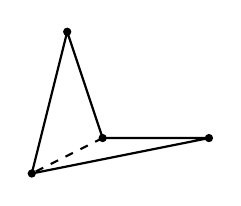
\begin{tikzpicture}[scale=0.45]

\draw[fill] (6,2) circle [radius=0.1];
\draw[fill] (3,2) circle [radius=0.1];
\draw[fill] (2,5) circle [radius=0.1];
\draw[fill] (1,1) circle [radius=0.1];
\draw[thick] (6,2) -- (3,2) -- (2,5) -- (1,1) -- (6,2);

\draw[dashed,thick] (3,2) -- (1,1);
\end{tikzpicture}
\end{center}
Per a un humà és clar quina de les línies és l'opció correcta, però la
situació és difícil per a un ordinador. Tanmateix, resulta que podem
resoldre el problema utilitzant un altre mètode més convenient per al
programador. Hi ha una fórmula general
\[x_1y_2-x_2y_1+x_2y_3-x_3y_2+x_3y_4-x_4y_3+x_4y_1-x_1y_4,\]
que calcula l'àrea d'un quadrilàter els vèrtexs del qual són
$(x_1,y_1)$, $(x_2,y_2)$, $(x_3,y_3)$ i $(x_4,y_4)$. Aquesta fórmula
és fàcil d'implementar, no hi ha casos especials, i fins i tot podem
generalitzar la fórmula a \emph{tots} els polígons.

\section{Nombres complexos}

\index{nombre complex} \index{punt} \index{vector}

Un \key{nombre complex} és un nombre de la forma $x+y i$, on $i =
\sqrt{-1}$ és la \key{unitat imaginària}. Una interpretació geomètrica
d'un nombre complex és que representa un punt bidimensional $(x,y)$ o
un vector des de l'origen fins a un punt $(x,y)$.

Per exemple, $4+2i$ es correspon amb el punt i el vector següents:


\begin{center}
\begin{tikzpicture}[scale=0.45]

\draw[->,thick] (-5,0)--(5,0);
\draw[->,thick] (0,-5)--(0,5);

\draw[fill] (4,2) circle [radius=0.1];
\draw[->,thick] (0,0)--(4-0.1,2-0.1);

\node at (4,2.8) {$(4,2)$};
\end{tikzpicture}
\end{center}


\index{complex@\texttt{complex}}

En C++ la classe de nombre complexos \texttt{complex} és útil per a
resoldre problemes geomètrics. Utilitzant la classe podem representar
punts i vectors com a nombres complexos, i la classe conté eines que
són útils en geometria.

En el codi següent, \texttt{C} és el tipus d'una coordenada i
\texttt{P} és el tipus d'un punt o vector. A més, el codi defineix
macros \texttt{X} i \texttt{Y} que es poden fer servir per a fer
referència a les coordenades $x$ i $y$.


\begin{lstlisting}
typedef long long C;
typedef complex<C> P;
#define X real()
#define Y imag()
\end{lstlisting}


Per exemple, el codi següent defineix un punt $p=(4,2)$ i imprimeix
les seves coordenades $x$ i $y$:


\begin{lstlisting}
P p = {4,2};
cout << p.X << " " << p.Y << "\n"; // 4 2
\end{lstlisting}


El codi següent defineix els vectors $v=(3,1)$ i $u=(2,2)$, i després
calcula la seva suma $s=v+u$.


\begin{lstlisting}
P v = {3,1};
P u = {2,2};
P s = v+u;
cout << s.X << " " << s.Y << "\n"; // 5 3
\end{lstlisting}


A la pràctica, un tipus de coordenada adequat sol ser \texttt{long
  long} (enter) o \texttt{long double} (nombre real). És bona idea fer
servir nombres enters sempre que sigui possible, perquè els càlculs
amb nombres enters són exactes. Si necessitem nombres reals, s'ha de
tenir en compte els errors de precisió a l'hora de comparar
nombres. Una manera segura de comprovar si els nombres reals $a$ i $b$
són iguals és comparar-los mitjançant $|a-b|<\epsilon$, on $\epsilon$
és un nombre petit (per exemple, $\epsilon=10^{-9}$).

\subsubsection*{Funcions}

En els exemples següents, el tipus de coordenades és \texttt{long double}.

La funció $\texttt{abs}(v)$ calcula la longitud $|v|$ d'un vector
$v=(x,y)$ mitjançant la fórmula $\sqrt{x^2+y^2}$. La funció també es
pot utilitzar per calcular la distància entre els punts $(x_1,y_1)$ i
$(x_2,y_2)$, perquè aquesta distància és igual a la longitud del
vector $(x_2-x_1,y_2-y_1)$.

El codi següent calcula la distància entre els punts $(4,2)$ i $(3,-1)$:
\begin{lstlisting}
P a = {4,2};
P b = {3,-1};
cout << abs(b-a) << "\n"; // 3.16228
\end{lstlisting}


La funció $\texttt{arg}(v)$ calcula l'angle d'un vector $v=(x,y)$
respecte a l'eix x. La funció dóna l'angle en radians, on $r$ radians
són $180 r/\pi$ graus. L'angle d'un vector que apunta cap a la
dreta és 0, i els angles disminueixen en sentit horari i augmenten en
sentit contrari.

La funció $\texttt{polar}(s,a)$ construeix un vector la longitud del
qual és $s$ i que apunta a un angle $a$. Un vector es pot girar per un
angle $a$ multiplicant-lo per un vector de longitud 1 i d'angle $a$.

El codi següent calcula l'angle del vector $(4,2)$, el gira $1/2$
radians en sentit contrari a les agulles del rellotge i després torna
a calcular l'angle:


\begin{lstlisting}
P v = {4,2};
cout << arg(v) << "\n"; // 0.463648
v *= polar(1.0,0.5);
cout << arg(v) << "\n"; // 0.963648
\end{lstlisting}


\section{Punts i línies}

\index{producte creuat}

El \key{producte creuat} $a \times b$ dels vectors $a=(x_1,y_1)$ i
$b=(x_2,y_2)$ es calcula mitjançant la fórmula $x_1 y_2 - x_2 y_1$. El
producte creuat ens indica si $b$ gira a l'esquerra (valor positiu),
no gira (zero) o gira a la dreta (valor negatiu) quan es col·loca
directament després de $a$.

La següent imatge il·lustra els casos anteriors:
\begin{center}
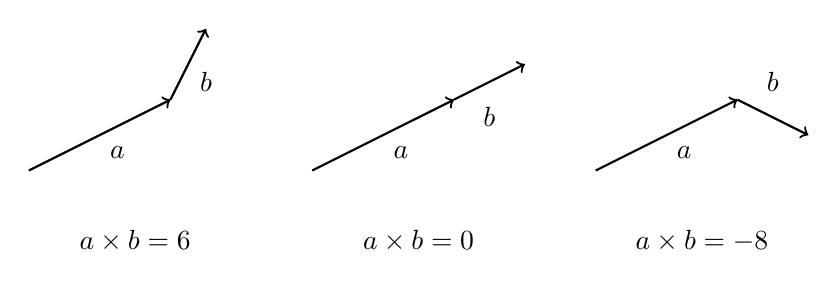
\begin{tikzpicture}[scale=0.45]

\draw[->,thick] (0,0)--(4,2);
\draw[->,thick] (4,2)--(4+1,2+2);

\node at (2.5,0.5) {$a$};
\node at (5,2.5) {$b$};

\node at (3,-2) {$a \times b = 6$};

\draw[->,thick] (8+0,0)--(8+4,2);
\draw[->,thick] (8+4,2)--(8+4+2,2+1);

\node at (8+2.5,0.5) {$a$};
\node at (8+5,1.5) {$b$};

\node at (8+3,-2) {$a \times b = 0$};

\draw[->,thick] (16+0,0)--(16+4,2);
\draw[->,thick] (16+4,2)--(16+4+2,2-1);

\node at (16+2.5,0.5) {$a$};
\node at (16+5,2.5) {$b$};

\node at (16+3,-2) {$a \times b = -8$};
\end{tikzpicture}
\end{center}


\noindent Per exemple, en el primer cas $a=(4,2)$ i $b=(1,2)$. El codi
següent calcula el producte creuat amb la classe \texttt{complex}:


\begin{lstlisting}
P a = {4,2};
P b = {1,2};
C p = (conj(a)*b).Y; // 6
\end{lstlisting}


El codi anterior funciona, perquè la funció \texttt{conj} nega la
coordenada $y$ d'un vector, i quan els vectors $(x_1,-y_1)$ i
$(x_2,y_2)$ es multipliquen junts, la coordenada $y$ del vector
resultant és $x_1 y_2 - x_2 y_1$.

\subsubsection{Ubicació d'un punt}

Els productes creuats es poden fer servir per comprovar si un punt es
troba al costat esquerre o dret d'una línia. Suposem que la línia
passa pels punts $s_1$ i $s_2$, mirant des de $s_1$ cap a $s_2$, i el
punt és $p$.

Per exemple, a la imatge següent, $p$ es troba al costat esquerre de
la línia:
\begin{center}
\begin{tikzpicture}[scale=0.45]
\draw[dashed,thick,->] (0,-3)--(12,6);
\draw[fill] (4,0) circle [radius=0.1];
\draw[fill] (8,3) circle [radius=0.1];
\draw[fill] (5,3) circle [radius=0.1];
\node at (4,-1) {$s_1$};
\node at (8,2) {$s_2$};
\node at (5,4) {$p$};
\end{tikzpicture}
\end{center}


El producte creuat $(p-s_1) \times (p-s_2)$ ens indica la ubicació del
punt $p$. Si el producte creuat és positiu, $p$ es troba al costat
esquerre, i si el producte creuat és negatiu, $p$ es troba al costat
dret. Finalment, si el producte creuat és zero, els punts $s_1$, $s_2$
i $p$ estan a la mateixa línia.

\subsubsection{Intersecció d'un segment amb una línia}

\index{intersecció de segment amb línia}

A continuació considerem el problema de comprovar si dos segments de
línia $ab$ i $cd$ es tallen. Els casos possibles són:

\textit{Cas 1:} Els segments de línia es troben a la mateixa línia i
se superposen. En aquest cas, hi ha un nombre infinit de punts
d'intersecció. Per exemple, a la imatge següent, tots els punts entre
$c$ i $b$ són punts d'intersecció:
\begin{center}
\begin{tikzpicture}[scale=0.9]
\draw (1.5,1.5)--(6,3);
\draw (0,1)--(4.5,2.5);
\draw[fill] (0,1) circle [radius=0.05];
\node at (0,0.5) {$a$};
\draw[fill] (1.5,1.5) circle [radius=0.05];
\node at (6,2.5) {$d$};
\draw[fill] (4.5,2.5) circle [radius=0.05];
\node at (1.5,1) {$c$};
\draw[fill] (6,3) circle [radius=0.05];
\node at (4.5,2) {$b$};
\end{tikzpicture}
\end{center}


Podem fer servir productes creuats per comprovar si tots els punts
estan a la mateixa línia. Després d'això, podem ordenar els punts i
comprovar si els segments de línia se superposen.

\textit{Cas 2:} Els segments de línia tenen un vèrtex comú que és
l'únic punt d'intersecció. Per exemple, a la imatge següent el punt
d'intersecció és $b=c$:


\begin{center}
\begin{tikzpicture}[scale=0.9]
\draw (0,0)--(4,2);
\draw (4,2)--(6,1);
\draw[fill] (0,0) circle [radius=0.05];
\draw[fill] (4,2) circle [radius=0.05];
\draw[fill] (6,1) circle [radius=0.05];

\node at (0,0.5) {$a$};
\node at (4,2.5) {$b=c$};
\node at (6,1.5) {$d$};
\end{tikzpicture}
\end{center}


Aquest cas és fàcil de comprovar, perquè només hi ha quatre
possibilitats per al punt d'intersecció: $a=c$, $a=d$, $b=c$ i $b=d$.

\textit{Cas 3:} Hi ha exactament un punt d'intersecció que no és un
vèrtex de cap segment de línia. A la imatge següent, el punt $p$ és el
punt d'intersecció:
\begin{center}
\begin{tikzpicture}[scale=0.9]
\draw (0,1)--(6,3);
\draw (2,4)--(4,0);
\draw[fill] (0,1) circle [radius=0.05];
\node at (0,0.5) {$c$};
\draw[fill] (6,3) circle [radius=0.05];
\node at (6,2.5) {$d$};
\draw[fill] (2,4) circle [radius=0.05];
\node at (1.5,3.5) {$a$};
\draw[fill] (4,0) circle [radius=0.05];
\node at (4,-0.4) {$b$};
\draw[fill] (3,2) circle [radius=0.05];
\node at (3,1.5) {$p$};
\end{tikzpicture}
\end{center}


En aquest cas, els segments de línia es tallen exactament quan els dos
punts $c$ i $d$ es troben a diferents costats de la línia que passa
per $a$ i $b$, i els punts $a$ i $b$ es troben a diferents costats de
la línia que passa per $c$ i $d$. Podem fer servir productes creuats
per comprovar-ho.

\subsubsection{Distància d'un punt a una línia}

Una altra característica dels productes creuats és que l'àrea d'un
triangle es pot calcular mitjançant la fórmula
\[\frac{| (a-c) \times (b-c) |}{2},\]
on $a$, $b$ i $c$ són els vèrtexs del triangle. Amb això podem
derivar una fórmula per calcular la distància més curta entre un punt
i una recta. Per exemple, a la imatge següent, $d$ és la distància més
curta entre el punt $p$ i la línia que està definida pels punts $s_1$
i $s_2$:
\begin{center}
\begin{tikzpicture}[scale=0.75]
\draw (-2,-1)--(6,3);
\draw[dashed] (1,4)--(2.40,1.2);
\node at (0,-0.5) {$s_1$};
\node at (4,1.5) {$s_2$};
\node at (0.5,4) {$p$};
\node at (2,2.7) {$d$};
\draw[fill] (0,0) circle [radius=0.05];
\draw[fill] (4,2) circle [radius=0.05];
\draw[fill] (1,4) circle [radius=0.05];
\end{tikzpicture}
\end{center}


L'àrea del triangle els vèrtexs del qual són $s_1$, $s_2$ i $p$ es pot
calcular de dues maneres: és $\frac{1}{2} |s_2-s_1| d$ i $\frac{1}{2}
((s_1-p) \times (s_2-p))$. Per tant, la distància més curta és
\[ d = \frac{(s_1-p) \times (s_2-p)}{|s_2-s_1|} .\]


\subsubsection{Punt dins d'un polígon}

Considerem ara el problema de comprovar si un punt està situat dins o fora d'un polígon. Per exemple, a la imatge següent, el punt $a$ es troba dins del polígon i el punt $b$ està fora del polígon.


\begin{center}
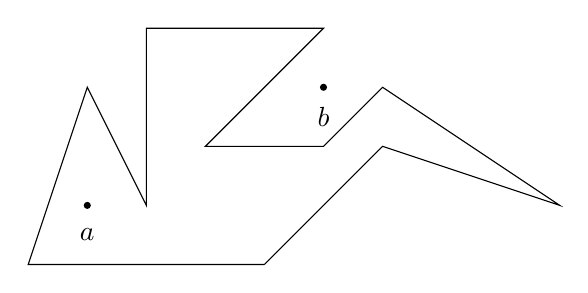
\begin{tikzpicture}[scale=0.75]
%\draw (0,0)--(2,-2)--(3,1)--(5,1)--(2,3)--(1,2)--(-1,2)--(1,4)--(-2,4)--(-2,1)--(-3,3)--(-4,0)--(0,0);
\draw (0,0)--(2,2)--(5,1)--(2,3)--(1,2)--(-1,2)--(1,4)--(-2,4)--(-2,1)--(-3,3)--(-4,0)--(0,0);

\draw[fill] (-3,1) circle [radius=0.05];
\node at (-3,0.5) {$a$};
\draw[fill] (1,3) circle [radius=0.05];
\node at (1,2.5) {$b$};
\end{tikzpicture}
\end{center}


Una manera convenient de resoldre el problema és enviar un \emph{raig}
des del punt en una direcció arbitrària i calcular el nombre de
vegades que toca la frontera del polígon. Si el nombre és senar, el
punt està dins del polígon, i si el nombre és parell, el punt està
fora del polígon.


\begin{samepage}
For example, we could send the following rays:
\begin{center}
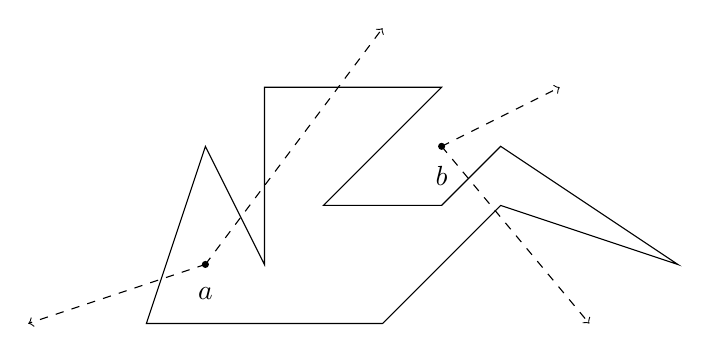
\begin{tikzpicture}[scale=0.75]
\draw (0,0)--(2,2)--(5,1)--(2,3)--(1,2)--(-1,2)--(1,4)--(-2,4)--(-2,1)--(-3,3)--(-4,0)--(0,0);

\draw[fill] (-3,1) circle [radius=0.05];
\node at (-3,0.5) {$a$};
\draw[fill] (1,3) circle [radius=0.05];
\node at (1,2.5) {$b$};

\draw[dashed,->] (-3,1)--(-6,0);
\draw[dashed,->] (-3,1)--(0,5);

\draw[dashed,->] (1,3)--(3.5,0);
\draw[dashed,->] (1,3)--(3,4);
\end{tikzpicture}
\end{center}
\end{samepage}


Els raigs de $a$ toquen 1 i 3 vegades la frontera del polígon, de
manera que $a$ es troba dintre. Els raigs de $b$ toquen 0 i 2 vegades
la frontera del polígon, de manera que $b$ es troba a fora.

\section{Àrea del polígon}

Una fórmula general per calcular l'àrea d'un polígon, de vegades
anomenada \key{fórmula de Gauss} o \key{fórmula de la llaçada} (de
cordons de sabates), és la següent: \index{fórmula de Gauss}
\[\frac{1}{2} |\sum_{i=1}^ {n-1} (p_i \times p_{i+1})| =
\frac{1}{2} |\sum_{i=1}^{n-1} (x_i y_{i+1} - x_{i+1} y_i)|, \] on $p_1
=(x_1,y_1)$, $p_2=(x_2,y_2)$, $\ldots$, $p_n=(x_n,y_n)$ és la
seqüència de vèrtexs adjacents a la frontera del polígon i el primer i
l'últim vèrtex són els mateixos, és a dir, $p_1=p_n$.

Per exemple, l'àrea del polígon
\begin{center}
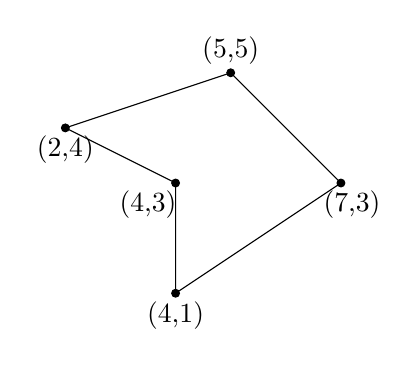
\begin{tikzpicture}[scale=0.7]
\filldraw (4,1.4) circle (2pt);
\filldraw (7,3.4) circle (2pt);
\filldraw (5,5.4) circle (2pt);
\filldraw (2,4.4) circle (2pt);
\filldraw (4,3.4) circle (2pt);
\node (1) at (4,1) {(4,1)};
\node (2) at (7.2,3) {(7,3)};
\node (3) at (5,5.8) {(5,5)};
\node (4) at (2,4) {(2,4)};
\node (5) at (3.5,3) {(4,3)};
\path[draw] (4,1.4) -- (7,3.4) -- (5,5.4) -- (2,4.4) -- (4,3.4) -- (4,1.4);
\end{tikzpicture}
\end{center}
és
\[\frac{|(2\cdot5-5\cdot4)+(5\cdot3-7\cdot5)+(7\cdot1-4\cdot3)+(4\cdot3-4\cdot1)+(4\cdot4-2\cdot3)|}{2} = 17/2.\]


La idea de la fórmula és passar pels trapezis un costat dels quals és
un costat del polígon i un altre costat es troba a la línia
horitzontal $y=0$. Per exemple:
\begin{center}
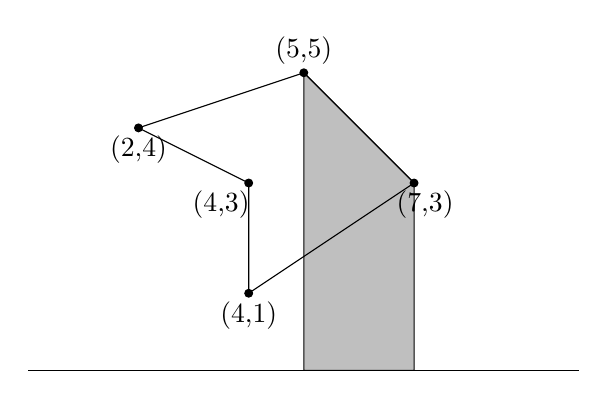
\begin{tikzpicture}[scale=0.7]
\path[draw,fill=lightgray] (5,5.4) -- (7,3.4) -- (7,0) -- (5,0) -- (5,5.4);
\filldraw (4,1.4) circle (2pt);
\filldraw (7,3.4) circle (2pt);
\filldraw (5,5.4) circle (2pt);
\filldraw (2,4.4) circle (2pt);
\filldraw (4,3.4) circle (2pt);
\node (1) at (4,1) {(4,1)};
\node (2) at (7.2,3) {(7,3)};
\node (3) at (5,5.8) {(5,5)};
\node (4) at (2,4) {(2,4)};
\node (5) at (3.5,3) {(4,3)};
\path[draw] (4,1.4) -- (7,3.4) -- (5,5.4) -- (2,4.4) -- (4,3.4) -- (4,1.4);
\draw (0,0) -- (10,0);
\end{tikzpicture}
\end{center}
L'àrea d'aquest trapezi és
\[(x_{i+1}-x_{i}) \frac{y_i+y_{i+1}}{2},\]
on els vèrtexs del polígon són $p_i$ i $p_{i+1}$. Si $x_{i+1}>x_{i}$,
l'àrea és positiva, i si $x_{i+1}<x_{i}$, l'àrea és negativa.

L'àrea del polígon és la suma de les àrees de tots aquests trapezis,
la qual cosa dóna la fórmula \[|\sum_{i=1}^{n-1} (x_{i+1}-x_{i}) \frac{y_i+y_{i+1}}{2}| = \frac{1}{2} |\sum_{i=1}^{n-1} (x_i y_{i+1} - x_{i+1} y_i)|.\]

Es pren el valor absolut de la suma perquè el seu valor pot ser
positiu o negatiu, depenent de si caminem en sentit horari o en sentit
contrari per la frontera del polígon.

\subsubsection{Teorema de Pick}

\index{Teorema de Pick}

\key{El teorema de Pick} proporciona una altra manera de calcular
l'àrea d'un polígon, sempre que tots els vèrtexs del polígon tinguin
coordenades enteres. Segons el teorema de Pick, l'àrea del polígon és
\[ a + b/2 -1,\]
on $a$ és el nombre de punts amb coordenades enteres dins del polígon
i $b$ és el nombre de punts amb coordenades enteres a la frontera del
polígon.

Per exemple, l'àrea del polígon
\begin{center}
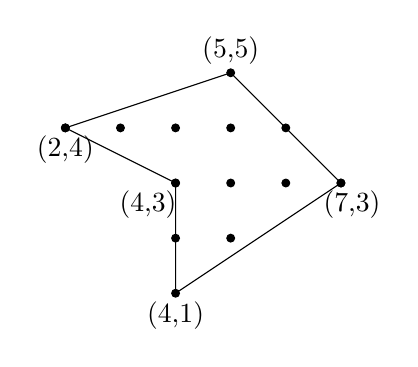
\begin{tikzpicture}[scale=0.7]
\filldraw (4,1.4) circle (2pt);
\filldraw (7,3.4) circle (2pt);
\filldraw (5,5.4) circle (2pt);
\filldraw (2,4.4) circle (2pt);
\filldraw (4,3.4) circle (2pt);
\node (1) at (4,1) {(4,1)};
\node (2) at (7.2,3) {(7,3)};
\node (3) at (5,5.8) {(5,5)};
\node (4) at (2,4) {(2,4)};
\node (5) at (3.5,3) {(4,3)};
\path[draw] (4,1.4) -- (7,3.4) -- (5,5.4) -- (2,4.4) -- (4,3.4) -- (4,1.4);

\filldraw (2,4.4) circle (2pt);
\filldraw (3,4.4) circle (2pt);
\filldraw (4,4.4) circle (2pt);
\filldraw (5,4.4) circle (2pt);
\filldraw (6,4.4) circle (2pt);

\filldraw (4,3.4) circle (2pt);
\filldraw (5,3.4) circle (2pt);
\filldraw (6,3.4) circle (2pt);
\filldraw (7,3.4) circle (2pt);

\filldraw (4,2.4) circle (2pt);
\filldraw (5,2.4) circle (2pt);
\end{tikzpicture}
\end{center}
és $6+7/2-1=17/2$.

\section{Funcions distància}

\index{funció distància} \index{Distància euclidiana} \index{Distància de Manhattan}

Una \key{funció distància} defineix la distància entre dos punts. La
funció distància habitual és la \key{distància euclidiana} on la
distància entre els punts $(x_1,y_1)$ i $(x_2,y_2)$ és
\[\sqrt{(x_2-x_1)^2+(y_2-y_1)^2}.\]
Una funció distància alternativa és la \key{Distància de Manhattan} on la distància entre els punts $(x_1,y_1)$ i $(x_2,y_2)$ és
\[|x_1-x_2|+|y_1-y_2|.\]

\begin{samepage}
Per exemple, considerem la imatge següent:
\begin{center}
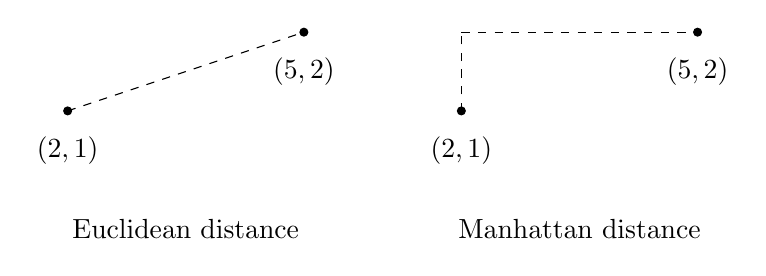
\begin{tikzpicture}

\draw[fill] (2,1) circle [radius=0.05];
\draw[fill] (5,2) circle [radius=0.05];

\node at (2,0.5) {$(2,1)$};
\node at (5,1.5) {$(5,2)$};

\draw[dashed] (2,1) -- (5,2);

\draw[fill] (5+2,1) circle [radius=0.05];
\draw[fill] (5+5,2) circle [radius=0.05];

\node at (5+2,0.5) {$(2,1)$};
\node at (5+5,1.5) {$(5,2)$};

\draw[dashed] (5+2,1) -- (5+2,2);
\draw[dashed] (5+2,2) -- (5+5,2);

\node at (3.5,-0.5) {Euclidean distance};
\node at (5+3.5,-0.5) {Manhattan distance};
\end{tikzpicture}
\end{center}
\end{samepage}
La distància euclidiana entre els punts és
\[\sqrt{(5-2)^2+(2-1)^2}=\sqrt{10}\]
i la distància de Manhattan és
\[|5-2|+|2-1|=4.\]
La imatge següent mostra regions que es troben a distància 1 del punt central, fent servir les distàncies euclidianes i de Manhattan:
\begin{center}
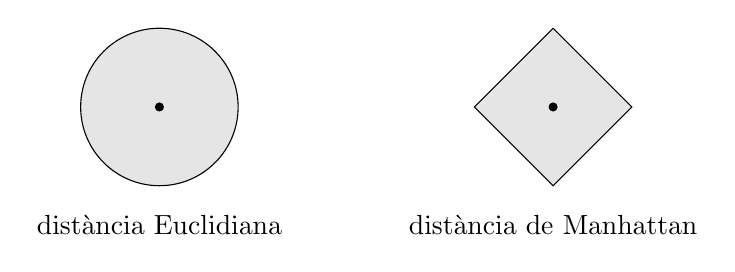
\begin{tikzpicture}

\draw[fill=gray!20] (0,0) circle [radius=1];
\draw[fill] (0,0) circle [radius=0.05];

\node at (0,-1.5) {dist\`ancia Euclidiana};

\draw[fill=gray!20] (5+0,1) -- (5-1,0) -- (5+0,-1) -- (5+1,0) -- (5+0,1);
\draw[fill] (5,0) circle [radius=0.05];
\node at (5,-1.5) {dist\`ancia de Manhattan};
\end{tikzpicture}
\end{center}


\subsubsection{Coordenades giratòries}

Alguns problemes són més fàcils de resoldre si es fa servir distàncies
de Manhattan en lloc de distàncies euclidianes. Per exemple,
considerem uel problema on se'ns donen $n$ punts en el pla
bidimensional i la nostra tasca és calcular la distància de
Manhattan màxima entre dos punts qualsevol.

Per exemple, considereu el següent conjunt de punts:
\begin{center}
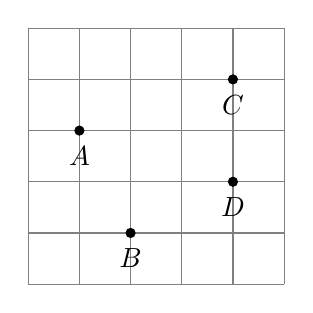
\begin{tikzpicture}[scale=0.65]
\draw[color=gray] (-1,-1) grid (4,4);

\filldraw (0,2) circle (2.5pt);
\filldraw (3,3) circle (2.5pt);
\filldraw (1,0) circle (2.5pt);
\filldraw (3,1) circle (2.5pt);

\node at (0,1.5) {$A$};
\node at (3,2.5) {$C$};
\node at (1,-0.5) {$B$};
\node at (3,0.5) {$D$};
\end{tikzpicture}
\end{center}
La distància de Manhattan màxima és 5, entre els punts $B$ i $C$:
\begin{center}
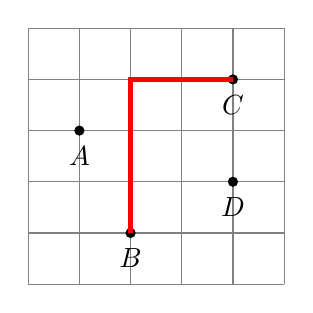
\begin{tikzpicture}[scale=0.65]
\draw[color=gray] (-1,-1) grid (4,4);

\filldraw (0,2) circle (2.5pt);
\filldraw (3,3) circle (2.5pt);
\filldraw (1,0) circle (2.5pt);
\filldraw (3,1) circle (2.5pt);

\node at (0,1.5) {$A$};
\node at (3,2.5) {$C$};
\node at (1,-0.5) {$B$};
\node at (3,0.5) {$D$};

\path[draw=red,thick,line width=2pt] (1,0) -- (1,3) -- (3,3);
\end{tikzpicture}
\end{center}


Una tècnica útil relacionada amb les distàncies de Manhattan és girar
totes les coordenades 45 graus de manera que un punt $(x,y)$
esdevingui $(x+y,y-x)$. Per exemple, després de girar els punts
anteriors, el resultat és:


\begin{center}
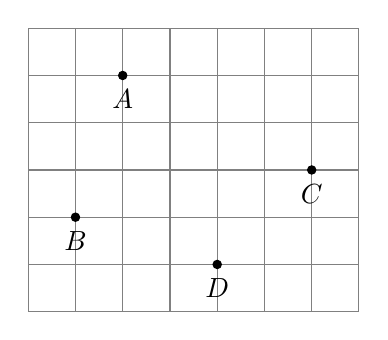
\begin{tikzpicture}[scale=0.6]
\draw[color=gray] (0,-3) grid (7,3);

\filldraw (2,2) circle (2.5pt);
\filldraw (6,0) circle (2.5pt);
\filldraw (1,-1) circle (2.5pt);
\filldraw (4,-2) circle (2.5pt);

\node at (2,1.5) {$A$};
\node at (6,-0.5) {$C$};
\node at (1,-1.5) {$B$};
\node at (4,-2.5) {$D$};
\end{tikzpicture}
\end{center}
I la distància màxima és la següent:
\begin{center}
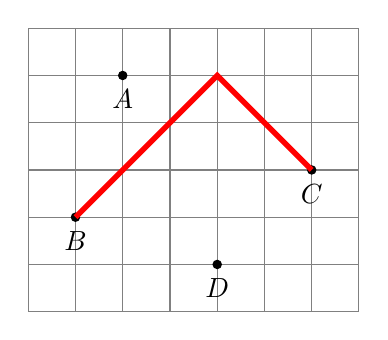
\begin{tikzpicture}[scale=0.6]
\draw[color=gray] (0,-3) grid (7,3);

\filldraw (2,2) circle (2.5pt);
\filldraw (6,0) circle (2.5pt);
\filldraw (1,-1) circle (2.5pt);
\filldraw (4,-2) circle (2.5pt);

\node at (2,1.5) {$A$};
\node at (6,-0.5) {$C$};
\node at (1,-1.5) {$B$};
\node at (4,-2.5) {$D$};

\path[draw=red,thick,line width=2pt] (1,-1) -- (4,2) -- (6,0);
\end{tikzpicture}
\end{center}


Considereu dos punts $p_1=(x_1,y_1)$ i $p_2=(x_2,y_2)$ les coordenades
girades dels quals són $p'_1=(x'_1,y'_1)$ i $p'_2=(x'_2, y'_2)$. Ara
hi ha dues maneres d'expressar la distància de Manhattan entre $p_1$ i
$p_2$:
\[|x_1-x_2|+|y_1-y_2| = \max(|x'_1-x'_2|,|y'_1-y'_2|)\]


Per exemple, si $p_1=(1,0)$ i $p_2=(3,3)$, les coordenades girades són
$p'_1=(1,-1)$ i $p'_2=(6,0 )$ i la distància de Manhattan és
\[|1-3|+|0-3| = \max(|1-6|,|-1-0|) = 5.\]


Les coordenades girades proporcionen una manera senzilla d'operar amb
distàncies de Manhattan, perquè podem considerar les coordenades x i y
per separat. Per maximitzar la distància de Manhattan entre dos punts,
hauríem de trobar dos punts les coordenades girades dels quals
maximitzin el valor de
\[\max(|x'_1-x'_2|,|y'_1-y'_2|).\]
Això és fàcil, perquè la diferència horitzontal o vertical de les
coordenades girades ha de ser màxima.


